%%%%%%
% HRI 2022 Final Project Report 
%%%%%%%

%%%%%%%%%%%%%%%%%%%%
% Abstract
%%%%%%%%%%%%%%%%%%%%
%%%%%
% Section 1: Abstract
%%%%%
\section{Abstract}
\begin{abstract}

Flight delays are a common issue that affect both airline operations and passengers. The purpose of this work is to investigate airline flight delays by analyzing historical airline flight data using two types of machine learning techniques: classification, to predict whether a flight will be delayed, and regression, to estimate delay duration. The dataset used in this project is publicly available from the U.S. Bureau of Transportation Statistics (BTS). Model comparison metrics include accuracy, precision, recall, F1 score, ROC-AUC, and RMSE.

The practical application of machine learning is evidenced by the example of an interactive application built using Streamlit. The app allows users to specify their trip parameters (departure city, destination city, month of travel, and delay risk threshold) to see how likely it is that an airline will be late on a particular route based on historical performance for that route and travel month. We compared a number of classification algorithms including logistic regression, random forest, gradient boosting, adaBoost, and extra trees; the gradient boosting algorithm provided the best overall accuracy of classification. For the regression problem, we created our own implementation of linear regression using NumPy and using the gradient descent method to estimate the duration of delays. Overall, this work demonstrates how machine learning can help transportation decision-makers in the real world by providing predictions of airlines, comparison of airlines, labeling of risks, and explanations of causes of delays in a user-friendly format.

\end{abstract}

\begin{IEEEkeywords}
flight delay prediction, machine learning, classification, regression, airline risk comparison, Streamlit, decision support
\end{IEEEkeywords}

%%%%%
% Section 2: Introduction
%%%%%
\section{Introduction}

Motivation: 
Flight delays remain a problem in the United States. Millions of passengers each year are affected by delays, and for some passengers, the impact can be significant. These delays can result in the loss of connecting flights, increased travelling costs, and disruptions to reliable travel, among other negative effects. Few tools provide predictive information about the potential for delays, but rather only provide historical data about airlines or do only real-time updates about flights. Furthermore, passengers usually do not understand why some flights are delayed, and therefore are not aware of their options to obtain a better travelling option. To address these challenges, we developed a mobile application that uses machine learning and allows the passengers to enter their departing city, arriving city, travel month, and delay risk threshold to generate historical route and month comparisons between airlines for the likelihood of a delay (both at take-off and upon arrival) along with the recommended airline based upon the lowest estimated delay risk to help passengers make better travel decisions.

Technical focus: We consider the problem as classification (predict whether or not a flight is going to be delayed) and regression (predict how long the delay is likely going to be). To determine complex relationships among multiple variables such as weather conditions, airline operation, and airport congestion, we have combined baseline and ensemble models including Logistic Regression, Random Forest, Gradient Boosting, AdaBoost, and Extra Trees. In our specific structure of delay, we have used five categories from BTS dataset which includes carrier delays, weather delays, national aviation system delays, security delays, and late aircraft delays; these core features allow us to analyze the historical delay patterns and help us predict delay risks and enable us to explain why delays occurred and give more meaningful suggestions to users.


Prior Work: Prior to this study, only machine learning methods or statistical models have been utilized in studying and predicting delays by analyzing multiple delays from previous events that could provide meaningful information about delay patterns. In addition, this study seeks to identify the major contributors of delays as well as enhance the overall accuracy of delay prediction. In contrast to all of the other studies published in the area of delay prediction have relied solely on individual outcome variables for purposes of predicting delays and did not provide a mechanism for extending findings from research to public domain applications. Therefore, our investigation enhances previous research by integrating delay prediction, delay cause explanation and user friendly decision support systems for assisting in making better decisions regarding delays.


Machine Learning Pipeline: The data collection, Exploratory Data Analysis (EDA) process, preprocessing, model training, model evaluation, and deployment are all part of the overall pipeline. The 2025 Bureau of Transportation Statistics (BTS) flight data were evaluated for all relevant attributes such as airline, route, and various types of delays to be included in the model created in this study. The various features that we used in our models to describe the delay are; Carrier delays, Weather delays, Delays caused by the National Airspace System (NAS), Delays caused by Security Issues, and Delays caused by Late Aircraft. We also conducted exploratory data analysis (EDA) to visualize how each attribute (the features that contribute to the delay) was distributed between all airlines, routes, travel distances and by each type of delay to help identify the patterns of delays for each type of delay. Once we identified the manner in which the EDA indicates missing data, encoded the categorical variables to use with our classification models, we created both a classification and a regression model in order to predict the probability that an airline flight will be delayed, along with the duration of the delay. In developing the classification model, we compared Logistic Regression, Random Forest, Gradient Boosting, AdaBoost, and Extra Trees using the traditional 80/20 train-test split method to identify the best-performing model. To create our regression model, we manually developed a Linear Regression model using NumPy and gradient descent to estimate the duration of the delay. To evaluate the performance of each model, we used multiple evaluation methods, including Accuracy, Precision, Recall, F1 Score, ROC-AUC, RMSE, and R². After identifying which classification model had the best performance throughout the evaluations, we incorporated the model output into a Streamlit application that will allow users to input the desired route and month of travel, along with a specified delay risk threshold, in order to retrieve airline delay risk comparisons, predicted delay duration, and the cause of the delay by airline.


Impact: This study aims to provide users with predictive analysis to assist in flight travel decision making, giving them a better understanding of the causes of travel delays. This knowledge will allow users to select more reliable travel options and optimize their trips. The study provides users with insight into the causes of delays on selected routes and within months, but there are a number of airports and potential data bias; hence, the results may not apply to all airport codes. Therefore, the study provides users with probability prediction estimates, risk labels, and delay-cause breakdowns to make the results easier for users to interpret and utilize for decision-making.

%%%%%
% Section 3: Background
%%%%%
\section{Background}

Flight delay prediction has been widely studied using both statistical and machine learning methods. Early work commonly used regression and classification models to predict delays based on historical flight data \cite{tang2021airline}. More recent studies have improved prediction performance by applying advanced methods, such as ensemble models and neural networks, to capture more complex relationships in the data \cite{jiang2020aviation}. Prior research has also shown that flight delays are influenced by multiple factors, including airline operations, departure time, and weather conditions \cite{choi2016weather}.

Recent literature further suggests that flight delays are not isolated events. Instead, delays can propagate across flights and through airport networks, which makes prediction more challenging \cite{chen2019chained, wu2019propagation}. Although these approaches often improve predictive accuracy, many of them rely on more complex models that are harder to interpret and apply in practice \cite{zoutendijk2021probabilistic}.

Our final approach is similar to prior  proposal in that it also uses historical flight data and machine learning to predict delay risk. However, our work differs from prior studies in two main ways. First, we compare multiple classification models and a regression model within a simpler and more interpretable framework. Second, we emphasize usability by integrating the results into an interactive Streamlit decision-support application. In our experiments, Gradient Boosting achieved the strongest classification performance among the tested models, while the front-end translated model outputs into airline-level risk comparisons, risk labels, and delay-cause explanations.
%%%%%
% Section 4: End-to-End ML Pipeline
%%%%%
\section{End-to-End ML Pipeline}

\subsection{Data Collection, Exploration \& Processing}

We use the 2025 BTS Airline On-Time Performance dataset obtained from the official U.S. Bureau of Transportation Statistics (BTS) TranStats Airline On-Time Performance Reporting download portal. This is an official U.S. government data source that provides public flight performance records, making it an appropriate and reliable dataset for our project. After merging the 12 monthly files for 2025, the dataset contains 7,001,619 rows and 22 columns, which provides broad coverage across airlines, origins, destinations, and dates. It is a structured tabular dataset with mixed data types. It includes temporal features (YEAR, QUARTER, MONTH, FL\_DATE), categorical features (OP\_UNIQUE\_CARRIER, ORIGIN, ORIGIN\_CITY\_NAME, ORIGIN\_STATE\_NM, DEST, DEST\_CITY\_NAME, DEST\_STATE\_NM), numerical features (DEP\_DELAY, DEP\_DELAY\_NEW, AIR\_TIME, DISTANCE, CARRIER\_DELAY, WEATHER\_DELAY, NAS\_DELAY, SECURITY\_DELAY, LATE\_AIRCRAFT\_DELAY, etc.), and a binary target-related variable (DEP\_DEL15). In total, the merged dataset has 10 float columns, 3 integer columns, and 9 object columns. 

We will use this dataset to build a model to investigate whether it is possible to predict flight delays in the United States based on weather, airline, departure or arrival cities, and operational factors. We will also use this to create a system that helps users choose more reliable airlines when traveling. The dataset already includes ground truth labels. We will use DEP\_DEL15 as the classification label and DEP\_DELAY\_NEW as the regression label.

During data cleaning, we examined the dataset shape, column types, missing values, and descriptive statistics. We also removed rows with missing values in the key delay-related columns: DEP\_DELAY, DEP\_DELAY\_NEW, DEP\_DEL15, CARRIER\_DELAY, WEATHER\_DELAY, NAS\_DELAY, SECURITY\_DELAY, and LATE\_AIRCRAFT\_DELAY. After cleaning, the analytical dataset contains 1,534,638 rows and 23 columns. The additional column is distance\_bucket, which was created from the continuous DISTANCE variable.

Our Exploratory Data Analysis (EDA) primarily serves the purposes of feature selection and task design. First, Figure~\ref{fig:target_distribution} illustrates the class distribution of the target variable, \texttt{DEP\_DEL15}, following data cleaning. Specifically, there are 321,689 flights that were either on time or delayed by less than 15 minutes, whereas 1,212,949 flights experienced delays of 15 minutes or more. This disparity indicates that accuracy alone is insufficient to comprehensively evaluate the model. Consequently, we incorporated precision, recall, F1 score, and ROC-AUC as supplementary evaluation metrics. Furthermore, Figure~\ref{fig:delay_group} demonstrates that flight delays are not merely a binary outcome; rather, the severity of delays varies significantly. Therefore, we also performed regression analysis to predict the expected delay duration. Additionally, Figure~\ref{fig:delay_factors} presents a comparative analysis of the overall distribution of various delay factors versus the distribution of factors associated with high-severity delays. We discovered that late aircraft delay, carrier delay, and NAS delay are the primary contributors to the accumulation of total delay time. Consequently, we included five specific features, \texttt{CARRIER\_DELAY}, \texttt{WEATHER\_DELAY}, \texttt{NAS\_DELAY}, \texttt{SECURITY\_DELAY}, and \texttt{LATE\_AIRCRAFT\_DELAY}, in our modeling process. Figure~\ref{fig:airline_delay} highlights the significant disparities among different airlines regarding both their overall delay rates and the average delay duration per flight. This establishes \texttt{OP\_UNIQUE\_CARRIER} as a crucial categorical feature within our model. It also provides the foundation for the design of our Streamlit application, wherein users can perform comparative analyses across different airlines and receive recommendations for airlines with relatively lower risk, based on the model's predictions regarding delay probability and expected delay duration. As illustrated in Figure~\ref{fig:distance_delay}, short-haul flights and long-haul flights exhibit distinct patterns of delay. Therefore, we retained \texttt{DISTANCE} as a numerical feature and further created a \texttt{distance\_bucket} variable to facilitate our subsequent analysis of flight distances. Finally, Figure~\ref{fig:delay_corr} reveals that the various causes of delays are not entirely mutually exclusive; indeed, certain types of delays frequently tend to occur simultaneously. Therefore, it is essential to employ multivariable machine learning models for comprehensive analysis.

\begin{figure}[t]
    \centering
    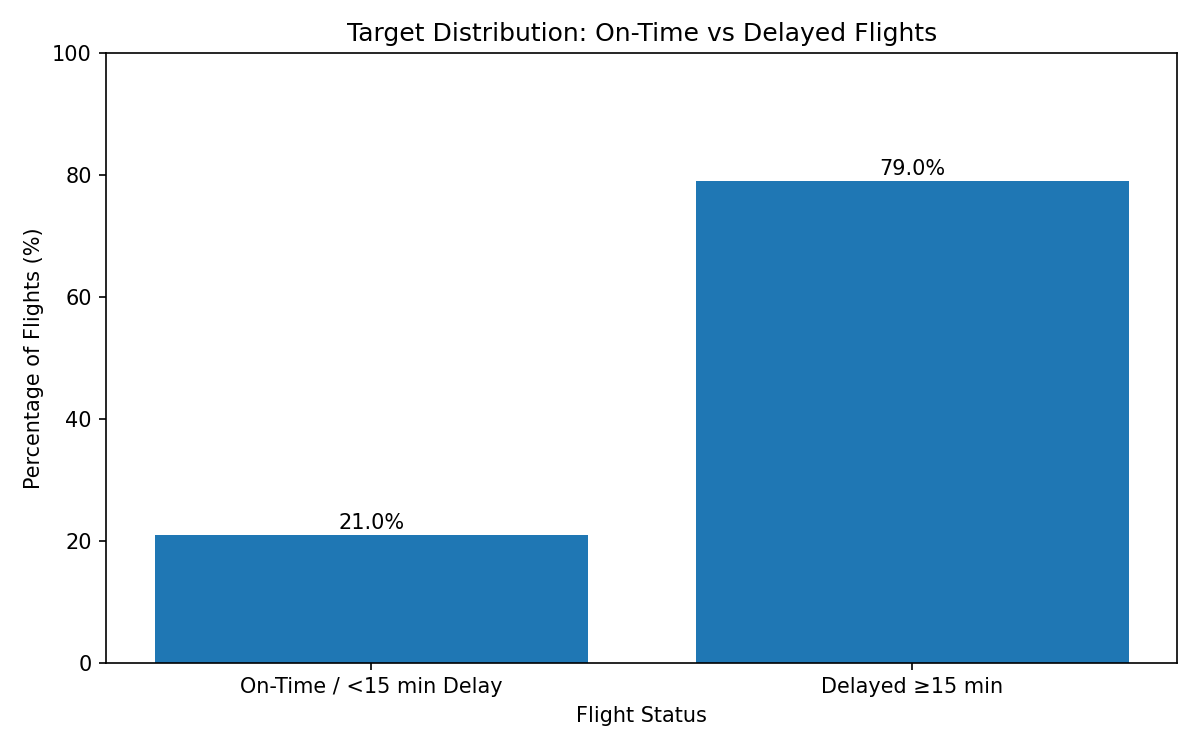
\includegraphics[width=0.85\linewidth]{Figures/target_distribution_dep_del15.png}
    \caption{Target distribution of DEP\_DEL15 in the cleaned dataset.}
    \label{fig:target_distribution}
\end{figure}

\begin{figure}[t]
    \centering
    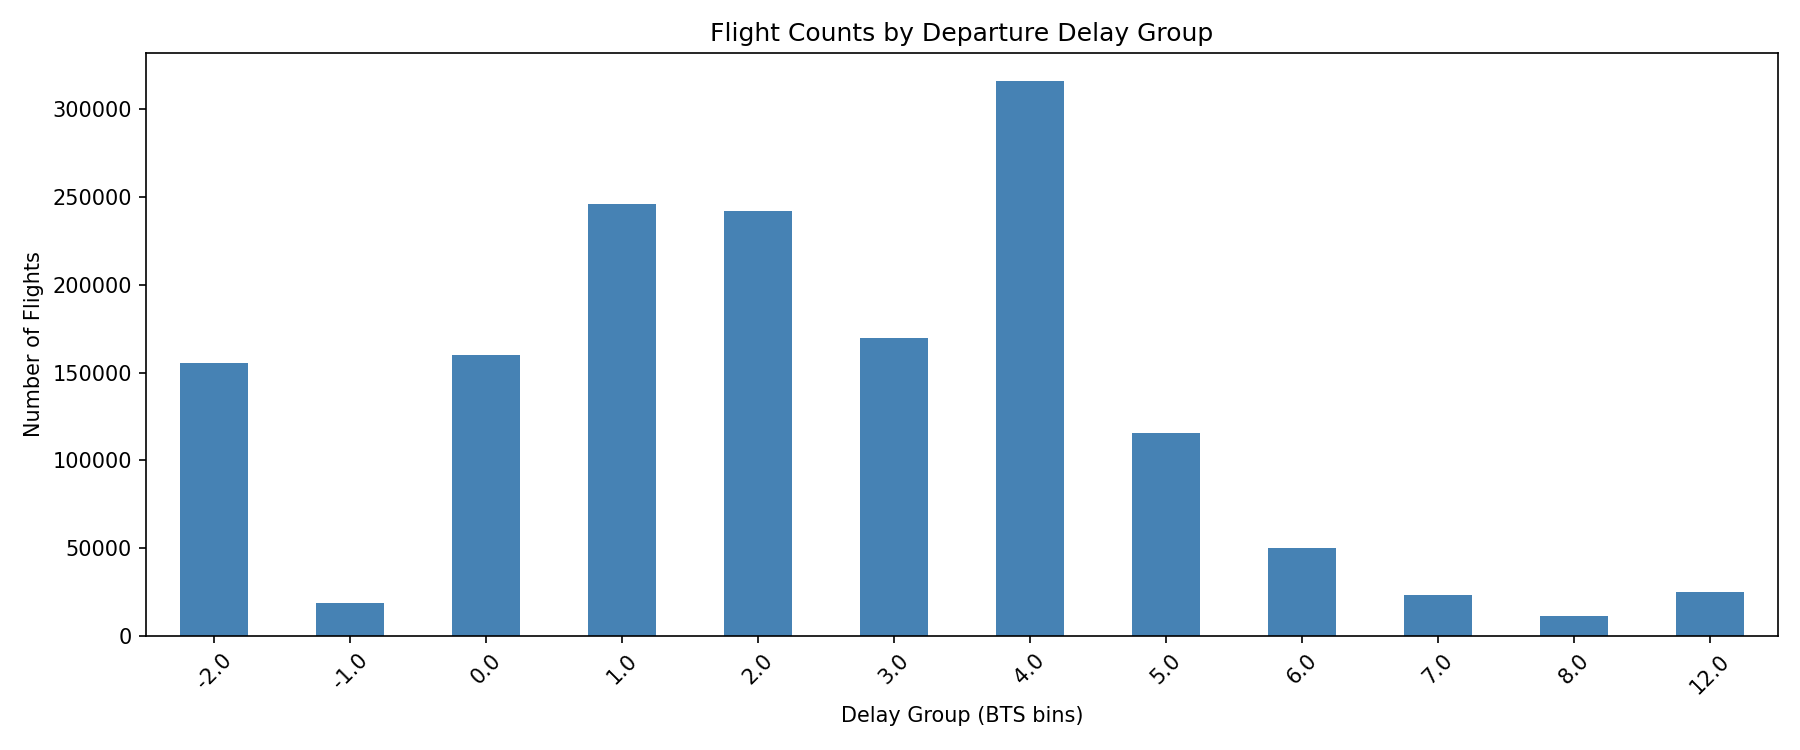
\includegraphics[width=0.9\linewidth]{Figures/flight_counts_by_delay_group.png}
    \caption{Flight counts by departure delay group.}
    \label{fig:delay_group}
\end{figure}

\begin{figure}[t]
    \centering
    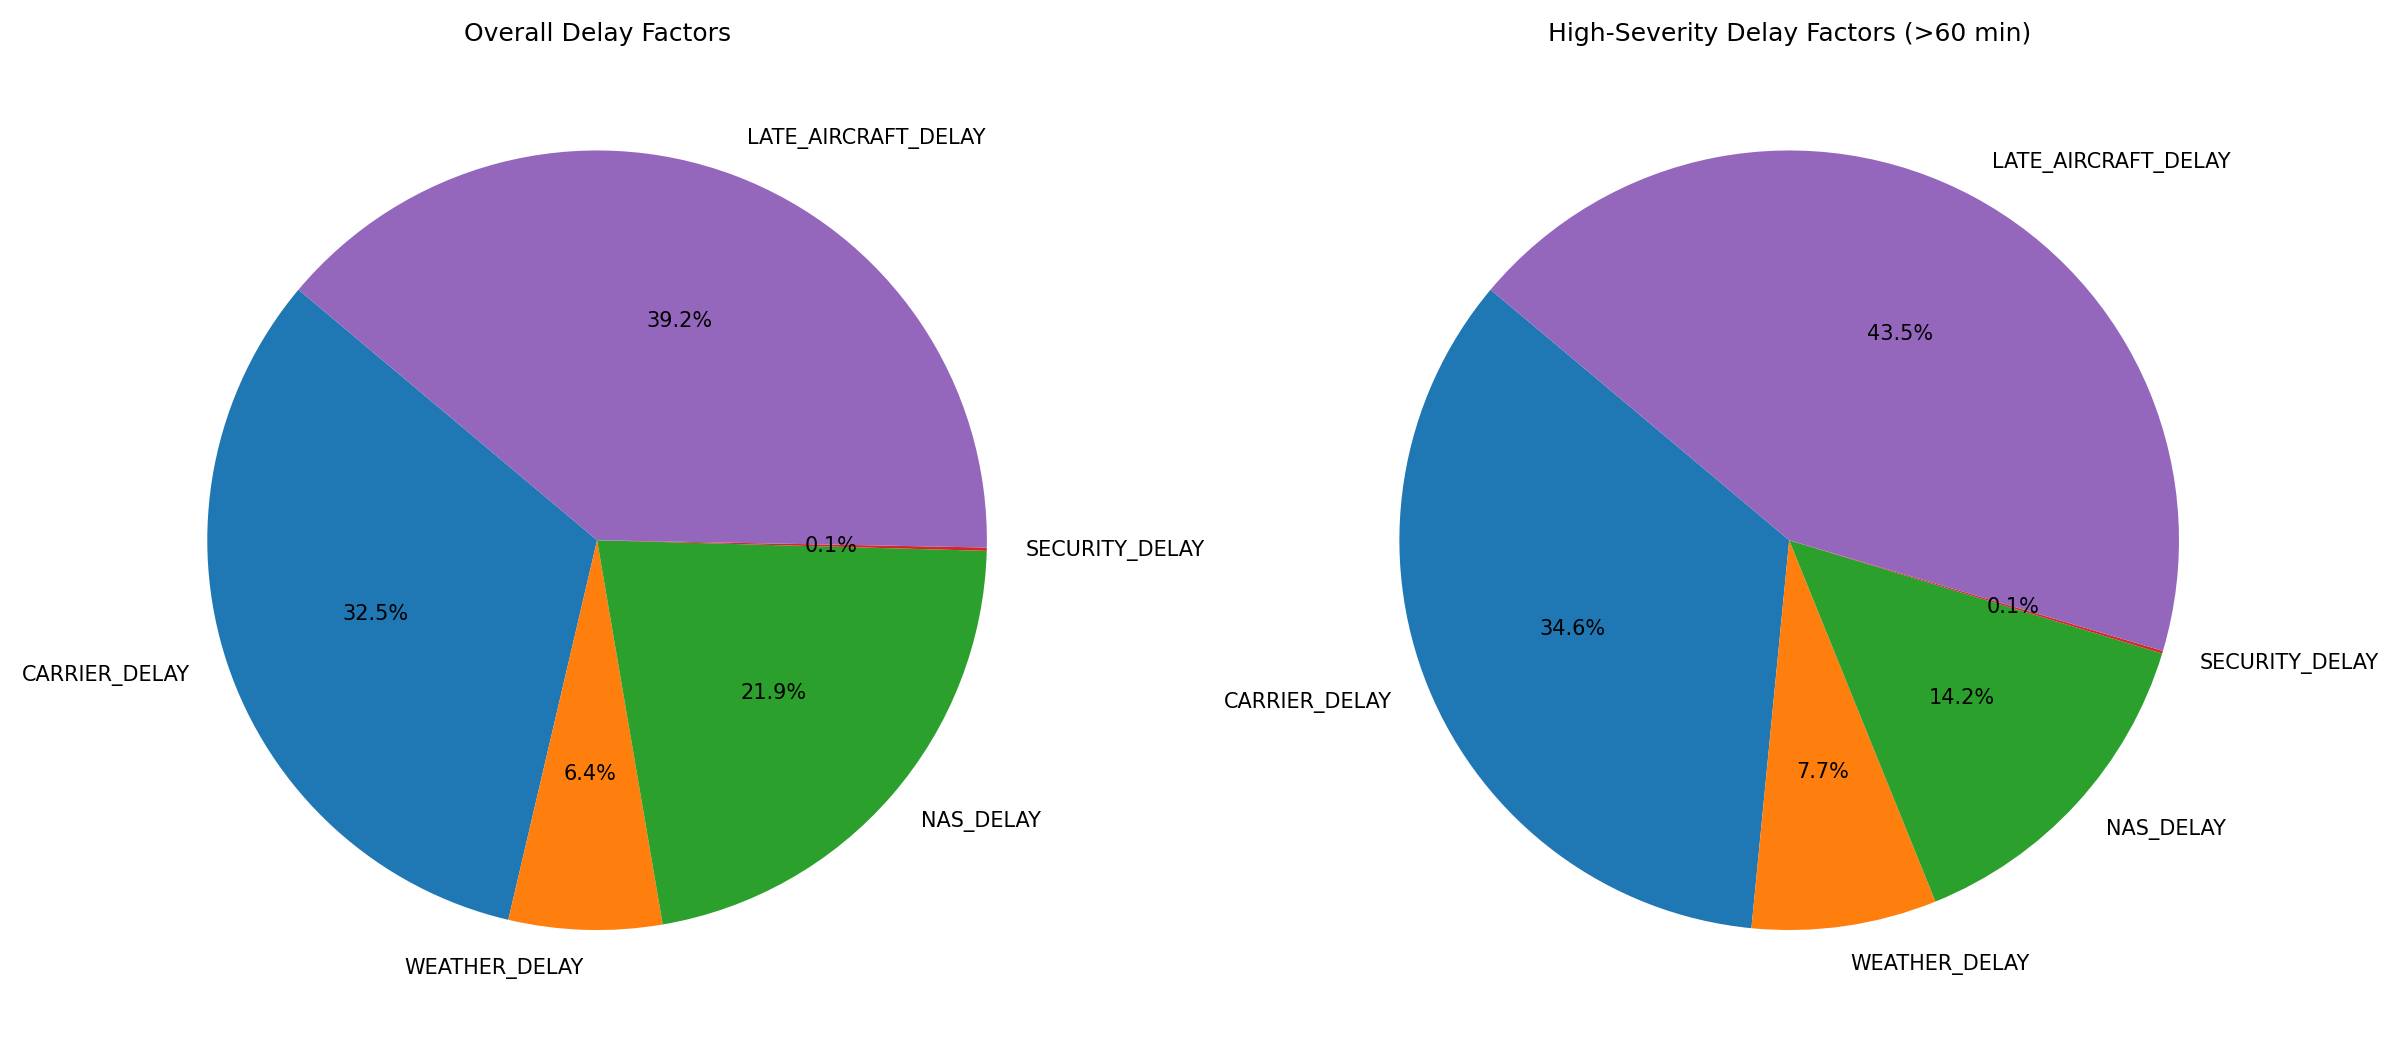
\includegraphics[width=\linewidth]{Figures/delay_factor_pie_charts.png}
    \caption{Overall and high-severity delay factor distributions.}
    \label{fig:delay_factors}
\end{figure}

\begin{figure}[t]
    \centering
    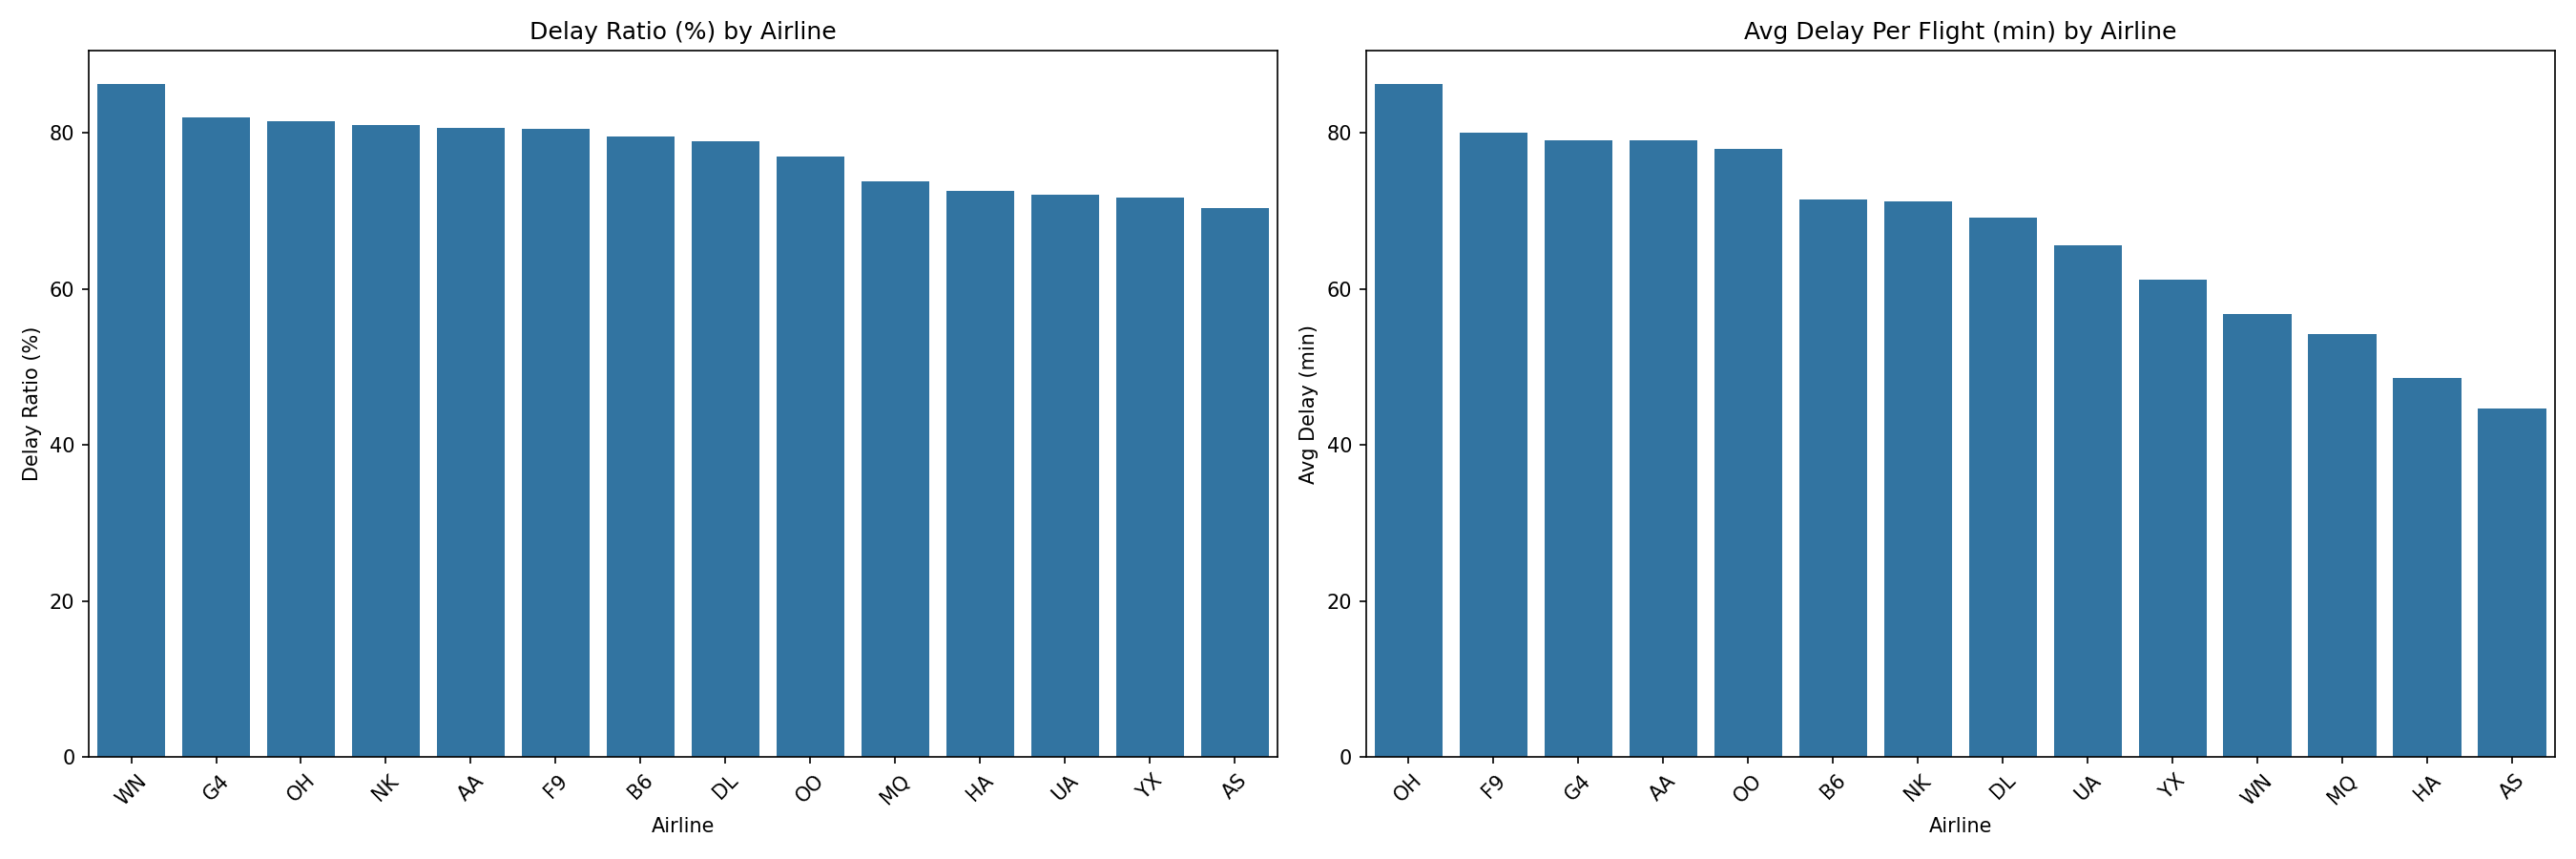
\includegraphics[width=\linewidth]{Figures/airline_delay_bar_charts.png}
    \caption{Airline-level delay ratio and average delay per flight.}
    \label{fig:airline_delay}
\end{figure}

\begin{figure}[t]
    \centering
    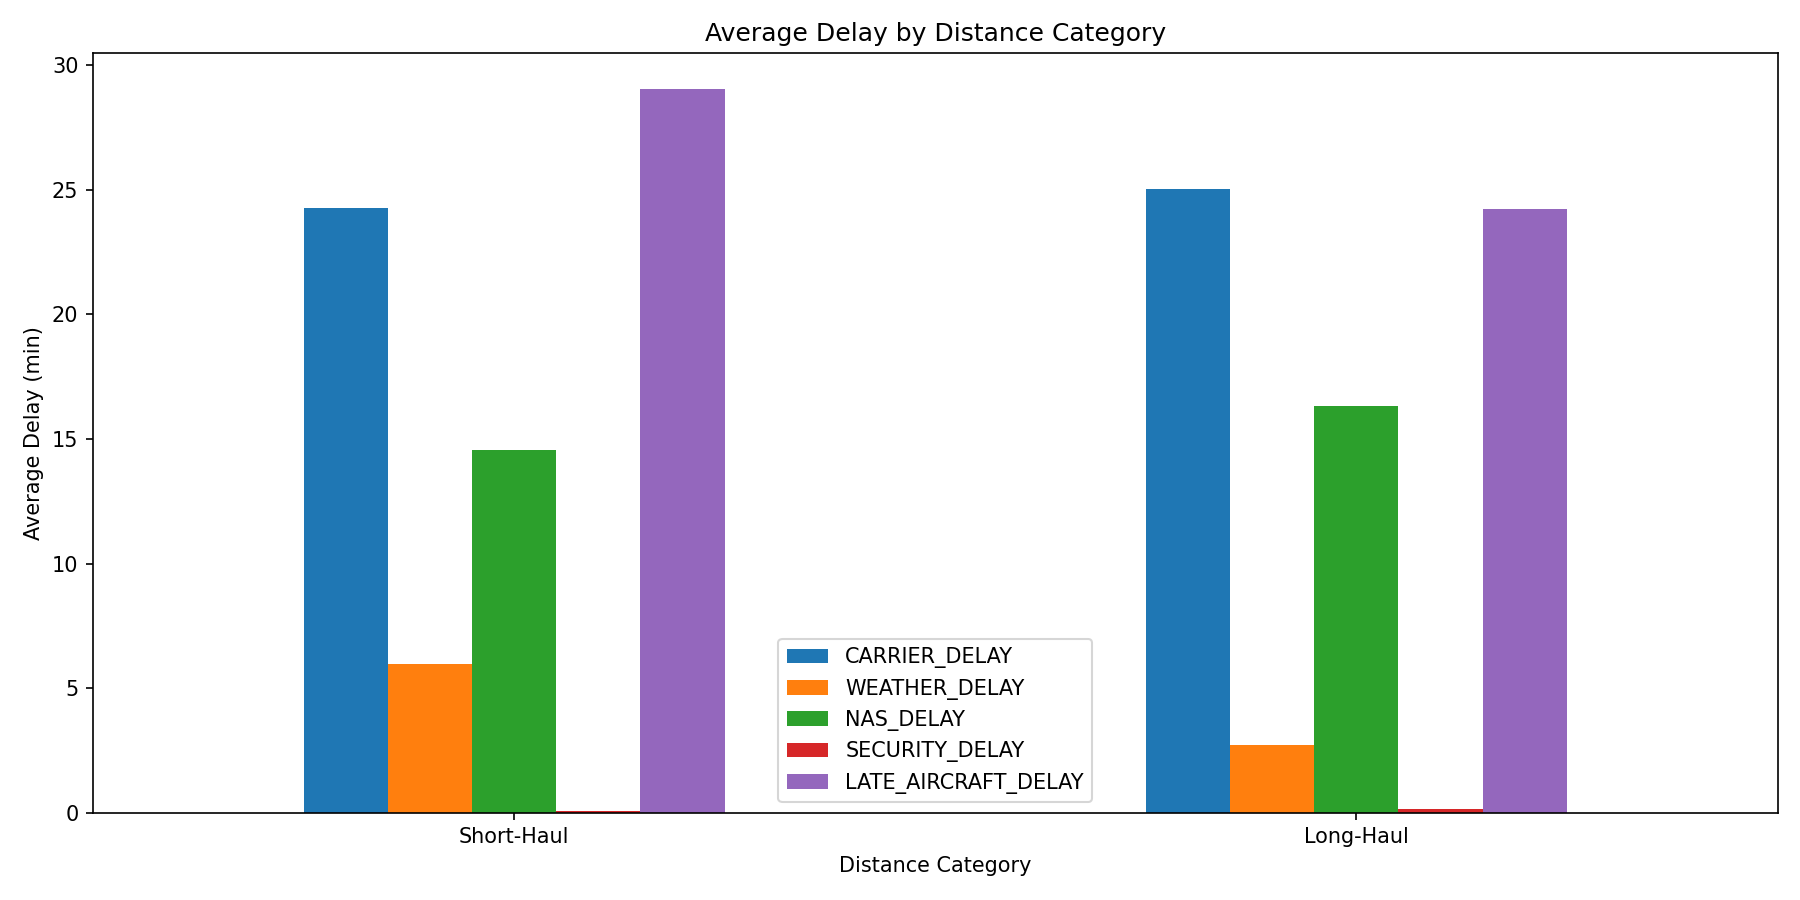
\includegraphics[width=0.95\linewidth]{Figures/short_vs_long_haul_delays.png}
    \caption{Average delay factors for short-haul and long-haul flights.}
    \label{fig:distance_delay}
\end{figure}

\begin{figure}[t]
    \centering
    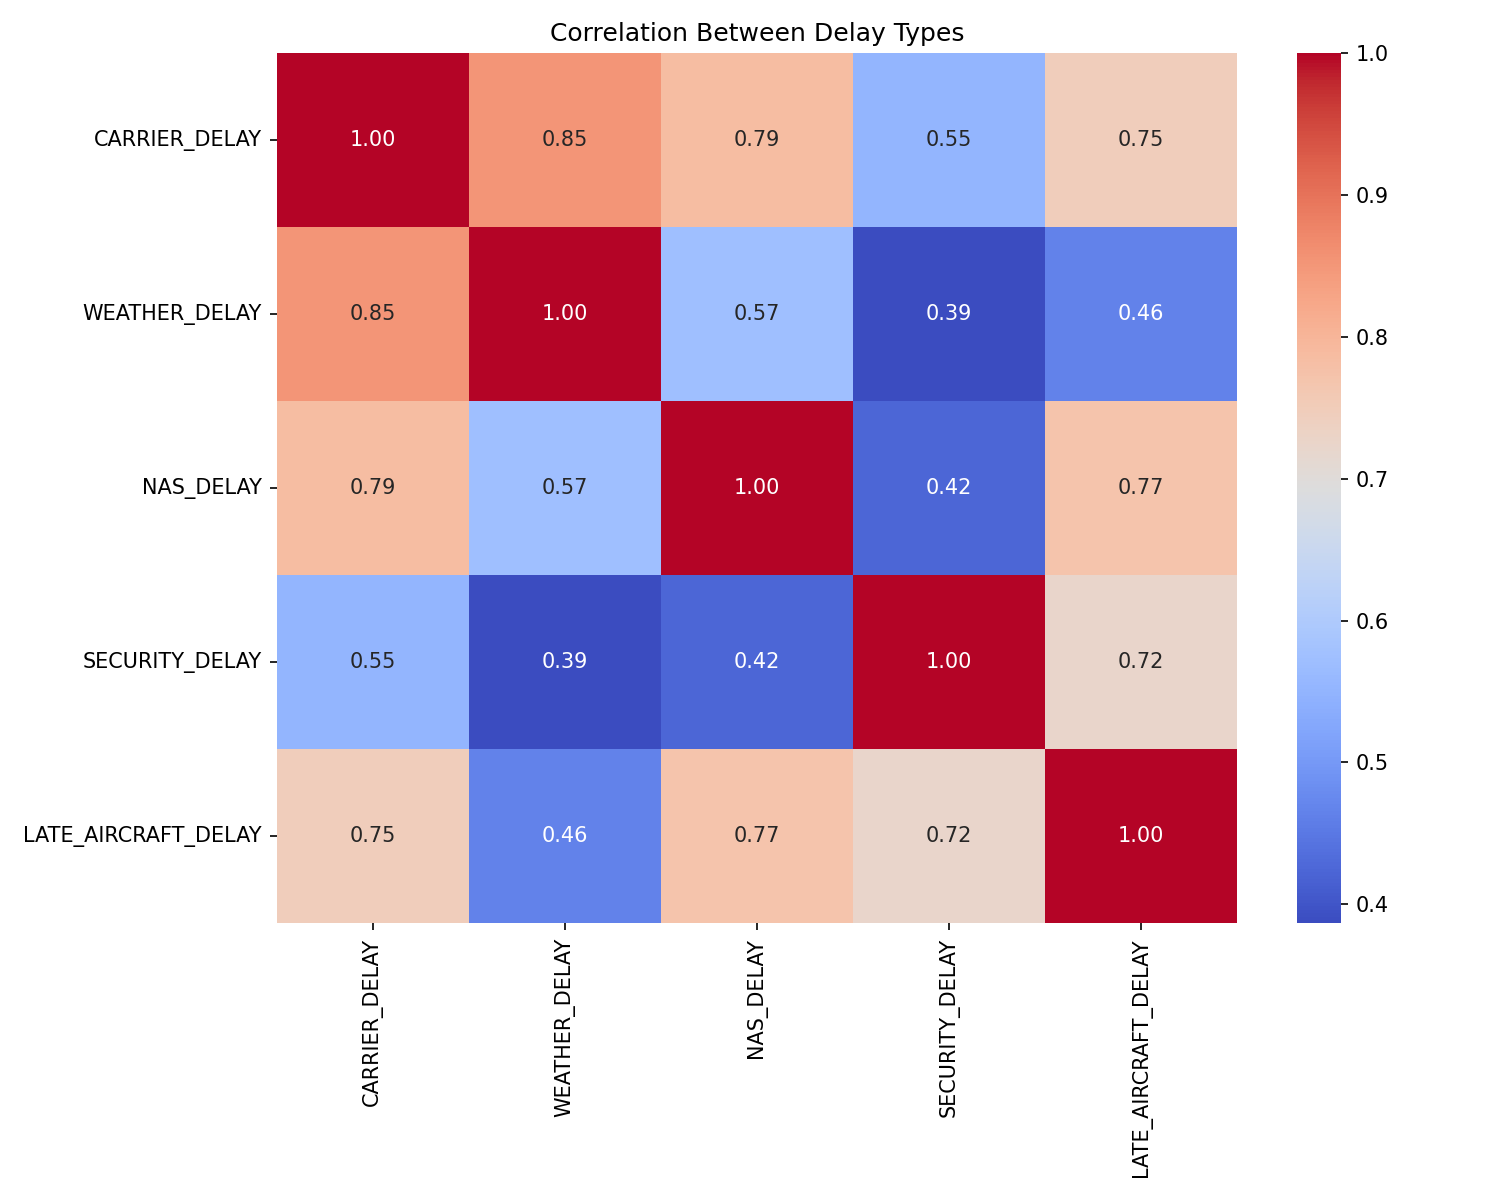
\includegraphics[width=0.85\linewidth]{Figures/correlation_heatmap_delay_types.png}
    \caption{Correlation heatmap of the five BTS delay-cause variables.}
    \label{fig:delay_corr}
\end{figure}

For preprocessing, we first handled missing data by removing rows with missing values in key delay-related columns. We then converted important numerical columns, including \texttt{MONTH}, \texttt{DISTANCE}, \texttt{AIR\_TIME}, \texttt{DEP\_DEL15}, and \texttt{DEP\_DELAY\_NEW}, into numeric format, and converted \texttt{DEP\_DEL15} into an integer classification label. Delay-duration variables, including \texttt{DEP\_DELAY\_NEW} and the five delay-cause variables, were clipped at 0 to ensure non-negative delay values. We also created \texttt{distance\_bucket} by discretizing \texttt{DISTANCE} into short-haul, medium-haul, and long-haul categories.

In the machine learning pipeline, numerical features are interpolated using the median and standardized using \texttt{StandardScaler}. Categorical features are interpolated using the mode and one-hot encoded. To reduce computational costs, we sampled 200,000 rows of data. Since the dataset is already quite large and severe delays significantly hinder our predictions and project progress, we did not perform dimensionality reduction, data augmentation, or outlier removal.

\subsection{Methods and Model Training} 

We formulated the project as two supervised learning tasks: classification and regression. For classification, the goal is to predict whether a flight will be delayed by at least 15 minutes using \texttt{DEP\_DEL15}, where 1 represents a delayed flight, and 0 represents an on-time flight or a flight delayed by less than 15 minutes. For regression, the goal is to predict the expected departure delay duration in minutes using \texttt{DEP\_DELAY\_NEW}.

For the classification task, we trained and compared five models: Logistic Regression, Random Forest, Gradient Boosting, AdaBoost, and Extra Trees. Logistic Regression was used as a simple baseline model. It estimates the probability of delay using the sigmoid function:

\[
P(y=1|x)=\frac{1}{1+e^{-(\beta_0+\beta^Tx)}}
\]

where \(x\) represents the input features and \(y\) represents the binary delay label. The tree-based ensemble models are suitable for this project because flight delays may depend on nonlinear relationships among airline, route, distance, month, and operational delay factors. Random Forest and Extra Trees combine multiple decision trees to reduce variance, while Gradient Boosting and AdaBoost build models sequentially to improve prediction errors. Based on the model comparison, Gradient Boosting achieved the best overall classification performance using F1 score, accuracy, and ROC-AUC, so it was selected as the final classification model.

For the regression task, we used Linear Regression implemented with NumPy and gradient descent to predict expected delay duration. The model predicts delay duration as:

\[
\hat{y}=\beta_0+\beta^Tx
\]

where \(x\) represents the regression input features and \(\hat{y}\) is the predicted delay duration in minutes. The model updates its weights by minimizing the prediction error between \(\hat{y}\) and the actual value of \texttt{DEP\_DELAY\_NEW}. Before training, the regression features were standardized, and model performance was evaluated using RMSE and \(R^2\).

The classification input features include \texttt{MONTH}, \texttt{OP\_UNIQUE\_CARRIER}, \texttt{ORIGIN}, \texttt{DEST}, \texttt{DISTANCE}, \texttt{AIR\_TIME}, \texttt{CARRIER\_DELAY}, \texttt{WEATHER\_DELAY}, \texttt{NAS\_DELAY}, \texttt{SECURITY\_DELAY}, and \texttt{LATE\_AIRCRAFT\_DELAY}. The regression input features include \texttt{MONTH}, \texttt{DISTANCE}, \texttt{AIR\_TIME}, \texttt{CARRIER\_DELAY}, \texttt{WEATHER\_DELAY}, \texttt{NAS\_DELAY}, \texttt{SECURITY\_DELAY}, and \texttt{LATE\_AIRCRAFT\_DELAY}. The classification output is a binary delay prediction, while the regression output is a continuous expected delay duration in minutes. We used an 80/20 train-test split for both tasks.


\subsection{Model Evaluation} 

For the classification task, we evaluated model performance using accuracy, precision, recall, F1 score, and ROC-AUC. Accuracy measures the overall proportion of correct predictions:

\[
Accuracy=\frac{TP+TN}{TP+TN+FP+FN}
\]

Precision measures how many flights predicted as delayed were actually delayed, while recall measures how many actual delayed flights were correctly identified:

\[
Precision=\frac{TP}{TP+FP}, \quad Recall=\frac{TP}{TP+FN}
\]

Since the cleaned dataset is imbalanced, F1 score is especially important because it balances precision and recall:

\[
F1=2\cdot\frac{Precision\cdot Recall}{Precision+Recall}
\]

ROC-AUC was also used to evaluate how well the model separates delayed and non-delayed flights across different probability thresholds. These metrics are suitable because accuracy alone can be misleading when one class is much larger than the other.

For the regression task, we used RMSE and \(R^2\). RMSE measures the average prediction error in minutes and penalizes larger errors more strongly:

\[
RMSE=\sqrt{\frac{1}{n}\sum_{i=1}^{n}(y_i-\hat{y}_i)^2}
\]

\(R^2\) measures how much variation in actual delay duration is explained by the model:

\[
R^2=1-\frac{\sum_{i=1}^{n}(y_i-\hat{y}_i)^2}{\sum_{i=1}^{n}(y_i-\bar{y})^2}
\]

For the experimental setup, we sampled 200,000 records from the cleaned dataset to reduce computational cost. For classification, we used an 80/20 train-test split with random\_state=42 and stratification, so the class distribution was preserved in both training and testing sets. All classification models used the same processed feature set and preprocessing pipeline. For regression, we trained the Linear Regression model on flights with positive delay duration, where DEP\_DELAY\_NEW \(>0\), and also used an 80/20 train-test split. The regression features were standardized using the training-set mean and standard deviation.

For classification experiments, we trained Logistic Regression, Random Forest, Gradient Boosting, AdaBoost, and Extra Trees. Logistic Regression used max\_iter=1000 and class\_weight='balanced'. Random Forest used n\_estimators=150, max\_depth=16, and min\_samples\_leaf=5. Gradient Boosting used n\_estimators=100, learning\_rate=0.1, and max\_depth=3. AdaBoost used n\_estimators=100 and learning\_rate=0.1. Extra Trees used n\_estimators=150, max\_depth=16, min\_samples\_leaf=5, and class\_weight='balanced'. For regression, the Linear Regression model was trained using gradient descent with learning\_rate=0.01 and epochs=1500.

To reduce overfitting, we evaluated all models on a held-out test set instead of only reporting training performance. For tree-based models, we limited model complexity using maximum tree depth and minimum samples per leaf. For boosting models, we used moderate values for the number of estimators and learning rate. To reduce underfitting, we compared both a simple baseline model and more flexible ensemble models, allowing us to select a model that captures nonlinear delay patterns while still being tested on unseen data.

\subsection{Results} 

Table~\ref{tab:classification_results} summarizes the classification results on the test set. Gradient Boosting achieved the best overall performance, with the highest accuracy, F1 score, and ROC-AUC. Logistic Regression achieved the highest precision, meaning that its delayed-flight predictions were usually correct. Random Forest achieved the highest recall, but its lower precision suggests that it tended to classify more flights as delayed. Extra Trees performed worst overall, with the lowest accuracy, recall, F1 score, and ROC-AUC. Therefore, Gradient Boosting was selected as the final classification model.

\begin{table}[t]
\centering
\caption{Classification model comparison on the test set.}
\label{tab:classification_results}
\resizebox{\linewidth}{!}{
\begin{tabular}{lccccc}
\hline
Model & Accuracy & Precision & Recall & F1 & ROC-AUC \\
\hline
Logistic Regression & 0.8851 & \textbf{0.9811} & 0.8716 & 0.9231 & 0.9636 \\
Random Forest & 0.8129 & 0.8097 & \textbf{0.9982} & 0.8941 & 0.9622 \\
Gradient Boosting & \textbf{0.9383} & 0.9603 & 0.9618 & \textbf{0.9611} & \textbf{0.9830} \\
AdaBoost & 0.9279 & 0.9573 & 0.9514 & 0.9543 & 0.9653 \\
Extra Trees & 0.6866 & 0.8890 & 0.6902 & 0.7771 & 0.7392 \\
\hline
\end{tabular}
}
\end{table}

For the regression task, Table~\ref{tab:regression_results} shows the delay-duration prediction results. The Linear Regression model achieved an RMSE of 17.18 minutes and an \(R^2\) of 0.9746. The mean predicted delay duration is very close to the mean actual delay duration, which suggests that the model captures the overall delay-duration pattern well.

\begin{table}[t]
\centering
\caption{Regression evaluation results on the test set.}
\label{tab:regression_results}
\begin{tabular}{lc}
\hline
Metric & Value \\
\hline
RMSE & 17.18 minutes \\
$R^2$ & 0.9746 \\
Mean actual delay & 77.69 minutes \\
Mean predicted delay & 77.80 minutes \\
\hline
\end{tabular}
\end{table}

Overall, the results show that our models can support both delay-risk classification and expected delay-duration prediction, aligning with the intention to provide practical flight decision support.

\subsection{Front-End (Streamlit)}

The front-end of the application was developed using Streamlit to provide an interactive and user-friendly airline delay risk comparison tool. The goal of the interface is to help users compare available airlines for a selected route and travel month based on historical delay patterns, predicted delay probability, expected delay duration, and delay-cause information. The final interface was designed as a single-page dashboard with a sidebar input panel and a main results area.

\subsubsection{Target Population}

The Streamlit Framework was used as the Front End to provide an interactive and user-friendly airport delay risk comparison system. The purpose of the interface is to assist users in comparing airlines for a specific route and travel month based on historical delay patterns, predicted probability of delay, estimated delay duration, and delay cause information. The final interface is a single page dashboard with an input panel on the side and a results area main.

\subsubsection{User Interface Layout}

Users of the service are people who travel in America, such as business travellers, students and tourists; all of whom wish to understand how much the airlines delay on average so they can make informed travel choices. Therefore, all users will likely have limited knowledge of technology or machine-learning and are likely to require the system be designed in a straightforward, intuitive visual manner that can easily be understood. Users will have a simple selection menu of basic trip details and all the processed data will provide a ranked list of available airlines, indicate how much each airline delays flights or provides visual examples to explain what to expect and be ready for when booking.

\begin{figure}[t]
\centerline{
\includegraphics[width=0.45\textwidth]{Figures/frontend_home.png}}
\caption{Home page input interface of the Streamlit application.}
\label{fig:frontend_home}
\end{figure}

Before the user runs a prediction, the main page displays overall airline delay statistics based on the historical dataset. After the user clicks the \textbf{Predict \& Compare} button, the dashboard updates to show airline-specific results for the selected route and month.

The results dashboard includes the following components:

\begin{itemize}

    \item \textbf{Lowest-Risk Airline Option:} Displays the airline with the lowest predicted delay probability among the available airlines. It also shows the predicted delay probability, expected delay duration, and risk level.

    \item \textbf{Recommendation Explanation Card:} Provides a short natural-language explanation of why the airline was selected, including the main estimated delay contributor.

    \item \textbf{Airline Comparison Table:} Ranks airlines by predicted delay probability and includes expected delay duration, risk level, and historical reliability.

    \item \textbf{Delay Risk and Expected Delay Charts:} Uses interactive bar charts to compare delay probability and expected delay duration across airlines. The delay probability chart also includes the user-selected risk threshold line.

    \item \textbf{Delay Cause Breakdown:} Shows the main delay contributors for the selected airline using a donut chart and a supporting bar chart for average delay minutes by cause.

\end{itemize}

\begin{figure}[t]
\centerline{
\includegraphics[width=0.45\textwidth]{Figures/frontend_results.png}}
\caption{Results dashboard displaying prediction outputs and the lowest-risk airline option.}
\label{fig:frontend_results}
\end{figure}

\begin{figure}[t]
\centerline{
\includegraphics[width=0.45\textwidth]{Figures/frontend_airline_comparison.png}}
\caption{Airline comparison table with delay probability and reliability ratings.}
\label{fig:frontend_airline_comparison}
\end{figure}

This layout helps users move from a high-level recommendation to more detailed comparisons and explanations.

\subsubsection{User Inputs and Outputs}

The application uses structured input widgets in the sidebar:

\begin{itemize}
    \item Dropdown menu for selecting departure city
    \item Dropdown menu for selecting arrival city
    \item Dropdown menu for selecting travel month
    \item Slider for selecting delay risk threshold
    \item A button labeled \textit{``Predict \& Compare''} to trigger the comparison
\end{itemize}

After the user submits the inputs, the application generates several outputs:

\begin{itemize}
    \item Predicted delay probability for each available airline
    \item Expected delay duration in minutes
    \item Risk level based on the user-selected threshold
    \item Lowest-risk airline option
    \item Ranked airline comparison table
    \item Interactive delay probability and expected delay charts
    \item Delay-cause breakdown for the selected airline
    \item A short explanation of why the option was selected
\end{itemize}

These outputs are designed to make the prediction results easier to interpret and more useful for decision-making.

\subsubsection{Front-End and Back-End Integration}

Through the use of cached data-loading and model-training functions, the application associates the front end (the user interface) and back end (the data and models) in order to use both together to create a working application. When a user clicks "Predict and Compare," Streamlit passes out to the back end all user's selections of departure city, arrival city, travel month, and risk threshold in order to build a workflow based on that information.

The backend initially filters the historical BTS data by selected route/mo. If no exact matches for the route and month are available, the application defaults to broader historical airline data. The backend then estimates delay probability, estimated delay duration and average delay cause for each available airline. The results are returned to the frontend as recommendation cards, an airline comparison table, interactive charts and a breakdown of delay causes as shown in Figures~\ref{fig:frontend_results},~\ref{fig:frontend_airline_comparison},~\ref{fig:frontend_delay_chart}, and~\ref{fig:frontend_delay_causes}.

\begin{figure}[t]
\centerline{
\includegraphics[width=0.45\textwidth]{Figures/frontend_delay_chart.png}}
\caption{Interactive bar charts comparing delay probability and expected delay duration across airlines.}
\label{fig:frontend_delay_chart}
\end{figure}

\begin{figure}[t]
\centerline{
\includegraphics[width=0.45\textwidth]{Figures/frontend_delay_causes.png}}
\caption{Delay-cause breakdown for the selected airline using a donut chart and supporting bar chart.}
\label{fig:frontend_delay_causes}
\end{figure}

The backend decision logic will factor in the user-selected risk threshold as well. If there are airlines predicted to delay above the user-selected threshold, these airlines are classified as "High Risk" while those below that threshold are classified as "Acceptable Risk." If there are no airlines available that are below your selected risk threshold, the application will still show the airline with the lowest risk while also alerting the user that their selected risk threshold was exceeded by all available airlines.


\subsubsection{Application Design Considerations}

The final interface was designed to be clear, concise, and actionable. Compared with the initial proposal design, the final version adds a user-adjustable risk threshold and a stronger explanation component. The dashboard also replaces static figures with interactive Streamlit and Altair visualizations, making the application feel more like a real decision-support tool rather than a notebook output.

The system is best understood as a historical route- and month-based airline risk comparison tool. It does not claim to provide real-time flight predictions. Instead, it helps users compare airlines using historical delay patterns, machine learning-based delay risk estimates, and interpretable delay-cause summaries. This makes the application more transparent and useful for everyday travel planning.


\section{Risk \& Mitigation}

While developing our application, we identified several potential risks associated with our data quality and interpretation. The BTS dataset contains many missing values in its delay-cause variables, meaning that removing rows that contain missing values could lead to overrepresenting the number of delayed flights. Consequently, we will view our results as based on a cleaned subset of delay-related data instead of the full flight population. Additionally, there is a possibility of data leakage since certain delay-cause variables will only be known after a flight has already been delayed. As a result, we will position our application as a historical, month and route-based comparison of airline risks rather than a real-time flight prediction application.

We looked into model risks regarding performance, run time and usability. Given that the cleaned data had more delayed flights than expected, some of these models may result in an overestimation of delayed flights. As a means of compensating for over-estimation and estimating model accuracy, we compared and evaluated several classification models on precision, recall, F1 score and ROC AUC; we sampled 200,000 rows of data as training data for each model and as a way to optimize run time through Streamlit's cached functions. Finally, we created a user interface with labels indicating risk as well as user-defined thresholds for distinguishing between "guaranteed" and "not guaranteed", explanatory cards detailing reasons/causes for the predictions made by the models and finally, an explanation of any delays that were included in the models.

\section{Conclusion}

In this project, we describes the development of a flight delay prediction and comparison application using historical BTS flight data is provided as well as how machine learning algorithms were utilized to evaluate predictions using classification and regression approaches to provide estimates of probability and duration of a flight delay for different airlines on a specified route and month. Predictions were then integrated with a user interface designed in Streamlit which allows users to compare different airline options based on interactive visualizations and explanation components.

In addition to improving model performance, our focus throughout the project was also to ensure interpretability and usability of our results. To achieve these two goals, we evaluated several different models using a number of measures (precision, recall, F1 score, and ROC AUC) and provided an end product that would allow users to view results that are clearly actionable by average travelers. Some of the features included in the application to help support users in understanding the rationale behind the provided recommendations were user-determined risk thresholds, the ability to view multiple airlines side-by-side in an airline comparison/table format, and breakdowns of delay-cause by airline as a means to assist users in understanding the relationship between airline delays and flight cancellations.

While the flight delay prediction application is built entirely on historical data, and therefore does not consider current weather and airport traffic conditions, it provides an example of how machine learning can be leveraged for practical support of user travel decision-making in a transparent and user-friendly manner. There remains ample opportunity for improvements to the application including the addition of real-time weather and airport traffic data; expanding the number of routes covered; and implementation of additional or more advanced predictive models to enhance the accuracy and personalization of the application.

%%%%%
% Section 5: Team Member Contribution
%%%%%
\section{Team Member Contribution}

Each team member contributes to both the technical and writing components of the project, with clearly defined responsibilities across front-end and back-end development.

\subsection{Technical Components}

Yufan Peng is responsible for data collection, model development, and model evaluation. Zhiying Huo focuses on exploratory data analysis (EDA) and back-end implementation. Xinrui Song contributes to model development and evaluation. Lin Wu is responsible for front-end development and supports exploratory analysis. Xinyi Huang focuses on literature review, exploratory data analysis, and model evaluation. This distribution ensures a balanced workflow across data processing, modeling, evaluation, and application development.

\subsection{Writing Components}

Yufan Peng is responsible for drafting the Introduction and Machine Learning Pipeline sections. Zhiying Huo contributes to the Data and Preprocessing description within the pipeline section. Xinrui Song focuses on the Model Training and Evaluation sections. Lin Wu is responsible for the Front-End (Streamlit application) description. Xinyi Huang contributes to the Background section and supports the Risk \& Mitigation and Expected Outcomes sections. All team members collaboratively review and revise the final report to ensure clarity, consistency, and completeness.

\bibliographystyle{ieee_fullname}
\bibliography{references}
